\graphicspath{{Chapter1/Figs/}}

\chapter{Introduction}
\label{chapter1}
      	
   \vspace*{\fill}\par
   \pagebreak

\section{The Sun}

    \begin{figure}
        \centering
        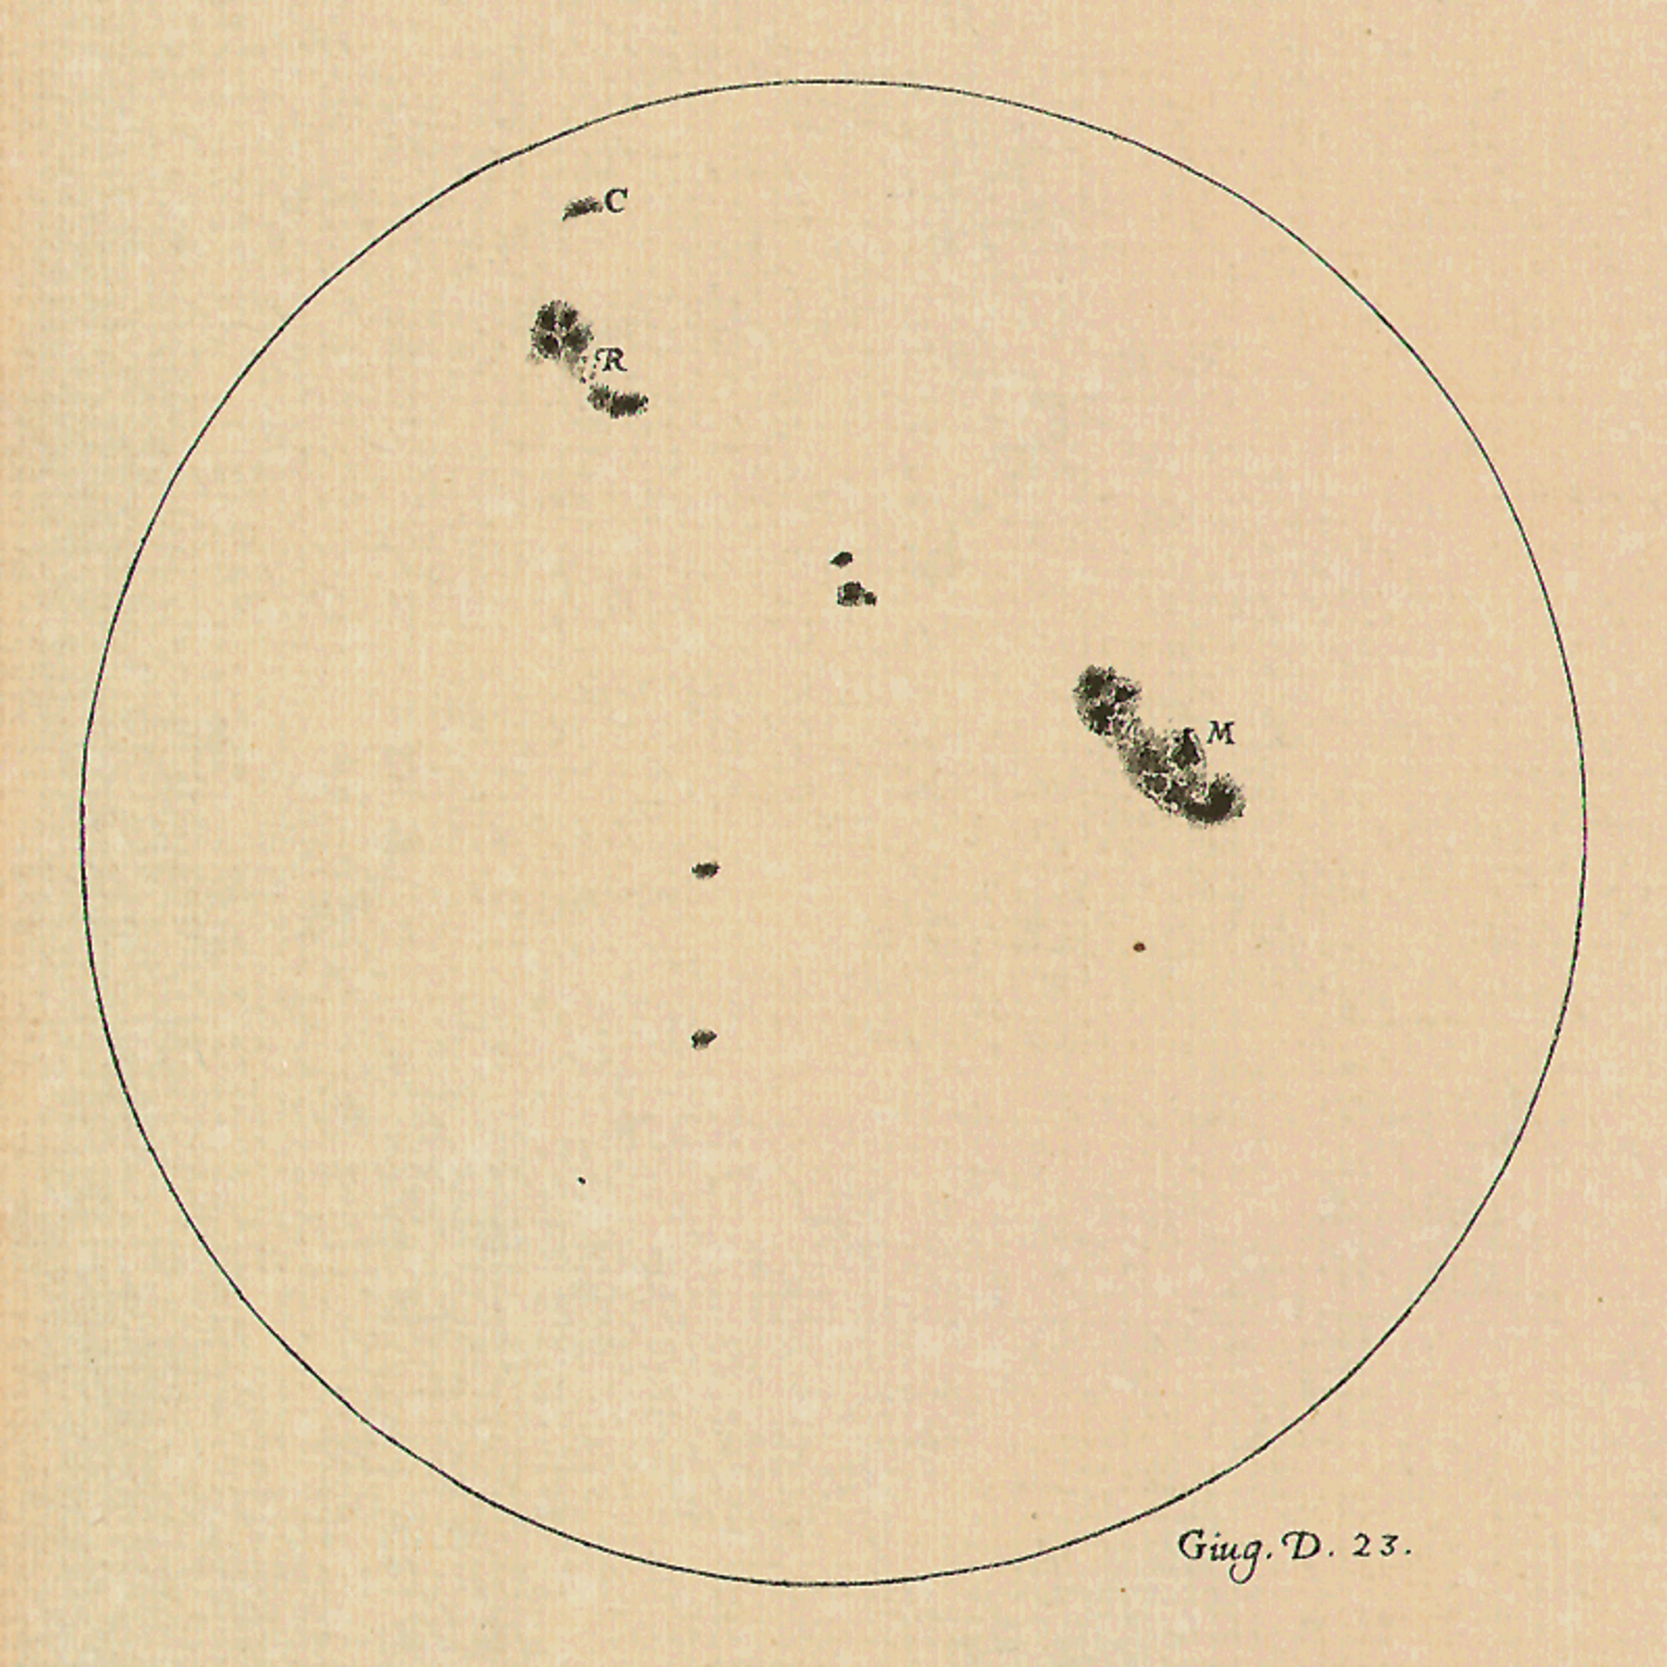
\includegraphics[width=\textwidth]{23_June_1613.pdf}
        \caption{
                 The creation of the telescope forever changed astronomy.
                 For example, here is a drawing of the solar surface by Galileo during the 17$^{\mathrm{th}}$ century. 
                 Here, the sunspot structure can be resolved.
                 The inner (umbra) and outer (penumbra) regions can be seen clearly.
                 Image credit goes to \cite{galileo}.
               }
        \label{fig:galileo}
    \end{figure}
     
    Our local star is known as the Sun and is a semi-common and uninteresting main sequence star if you happen to be an astrophysicist.
    However to the general public and more importantly solar physicists, it forms the backbone of their lives.
    From simply as mundane as waking up at sunrise, to making a long and (hopefully) successful career in solar physics.
    
    For early humans, it was as a giant bright ball in the sky that appeared to revolve around the Earth and it defied any human understanding at that time.
    Since the dawn of mankind, the mythology surrounding the Sun has been numerous.    
    From the New World, the Aztec's had a sun god called Tonatiuh. 
    Without constant human sacrifice (mainly their enemies), they believed that the Sun would not move through the sky.
    From the Far East, the Chinese originally had 10 suns who took turns moving through the sky. 
    However, these suns were mischievous and decided to all appear at the same time. 
    This made life utterly unbearable on Earth, so an archer bestowed with a unique bow shot down 9 of the suns, leaving the one sun we have today.
    From the Old World, the Greeks and Romans believed in Apollo who is the son of Zeus and Leto.
    He was known as the god of music, healing, light, truth and the Sun; a very busy god.
    With the decline of polytheism and the rise of monotheism, these gods and stories quickly became consigned to history. 
    For a review of solar mythologies, see \citet{mythbook}.
    
    The Sun had always been observed with the naked eye, sunspots have been visible and recorded by the ancient Chinese, further, many solar calenders were created to order human society.
    However, no systematic studies of the Sun had ever taken place.
    It was until the enlightenment in Europe which marked the start of a massive transformation of European society, in which the telescope was invented (among other things).
    This is the beginning of modern astronomy.
    
    The telescope was the instrument that allowed humanity's knowledge of our solar system to radically change.
    It was possible to observe the Sun in much greater detail for the first time.
    Galileo drew many full disc images of the Sun and Figure \ref{fig:galileo} is one such example. 
    With the telescope, the umbra and penumbra of sunspots was easily differentiated for the first time.
    Further, magnetic pores can be seen in the image.
    From here, many other discoveries were made such as the sunspot cycle, differential rotation and solar flares.
    With more time and a solar eclipse, layers of the solar atmosphere were finally observed, such as the chromosphere and the corona.
    The age of solar physics had finally begun.
    
    The scientific understanding of the Sun has advanced by leaps and bounds, especially during the past sixty years.
    This is mainly due to the launch of space missions, whether it was SkyLab or the numerous satellites now pointed at the Sun.
    The removal of the Earth's atmosphere was a decisive step, allowing the observation of spectral lines not possible on Earth and vastly improving the quality of observational data.
    The solar physics community is hard at work analysing the massive amount of data that is available and expanding our knowledge of the Sun.   
    However, there are still crucial challenges to overcome.
    They have in essence become the holy grails of solar physics: how the corona is heated and what is the dynamo process behind the solar magnetic field.

\subsection{The structure of the solar interior}

    The Sun's internal structure is divided into four sections; the core, the radiative zone, the tachocline and the convective zone.
    While we cannot see these regions directly, the process of helioseismology, much like seismology on Earth, has allowed humanity to come to grips with these layers and processes that occur within the Sun.
    Figure \ref{fig:Sun} showcases the multi-layered structure of the Sun.
    The image starts from the core, through the various interior layers until it reaches the solar atmosphere and the interplanetary medium.
    This picture of the Sun has built up over time as our understanding has improved with the use of more observations and complex mathematical models during the past 100 years.
    
    \begin{sidewaysfigure}
        \centering
        \includegraphics[width=\textwidth]{sun.pdf}
        \caption{
                A schematic diagram of the interior and external layers of the Sun.
                Also shown are several features that occur within the solar atmosphere; sunspots, granulation, flares and prominences.
                Image credit to \cite{sun_image}.
               }
        \label{fig:Sun}
    \end{sidewaysfigure}

\subsubsection{The core}

    The core is the beating heart of the Sun, the largest fusion reactor this side of Centaurus.
    The core has more than 60\% of the total mass of the Sun and extends roughly to 25\% of the total radius of the Sun.
    It has a density of around 150000 kg m$^{-3}$ and a temperature around 16 MK \citep{0004-637X-699-2-1403}.
    The fusion reactions occur due to the high pressure and temperatures that exist in the core, which are enough to force the hydrogen atoms together. 
    This process, which accounts for the vast majority of the energy generated, creates a range of high energy particles such as photons and neutrinos.
    
\subsubsection{The radiative zone}

    Due to the intense heat and the large pressure within this region, thermal radiation is the only mechanism able to transfer the heat generated by the core.
    The process of radiative transfer within the radiative zone happens on very small scales.
    Photons are emitted and absorbed on very short time-scales. 
    This means that it takes hundreds of thousands years for photons to exit this layer.
    The radiative zone extends to about 70\% of the solar radius \citep{cox1991solar}. 
        
\subsubsection{The tachocline}

    The tachocline is the region that separates the radiative zone and the convective zone.
    It is very thin, its width being only 0.04\% of the solar radius.
    It has been long hypothesised that the solar magnetic field is created within this layer via a dynamo process \citep{soward2005fluid}.

\subsubsection{The convection zone}

    From the tachocline, the temperature and pressure has decreased enough to allow the fully ionized molecules to retain some electrons and thus the opaqueness of the plasma increases.
    This traps part of the radiative energy from below setting up a temperature gradient sufficient enough to allow convection to take place.
    Thermal columns are created, which carry hot plasma to the surface of the Sun and once it cools, it sinks back to the base of the convection zone.
    This process is believed to cause gravity waves within the solar interior which have yet to be observed.
    The visible effect of convection is the solar granulation pattern that can be seen in white light images of the Sun.  
    The pattern consists of cells that have a rough hexagonal shape. 
    At the top of the convection zone, the temperature drops to 5700 K and the density to 0.0002 kg m$^{-3}$ \citep{gai2000sun}. 
    Within the convection zone, differential rotation is important.
    The Sun rotates not as a solid body as the Earth does but as a fluid as the Gas Giants do. 
    The rotation rate decreases from the equator where it is 25 days to around 34 days at the poles \citep{2000SoPh..191...47B}.
    Furthermore, the rotation rate varies with depth, until the tachocline is reached, where it rotates as a solid body \citep{Howe31032000}.
    
\subsection{The solar atmosphere}
 
    The solar atmosphere is quite unlike the Earth's.
    While they both have multiple layers, the characteristics are wildly different (as you would expect). 
    The top of the convection zone is the start of the first layer of the solar atmosphere.
    The reason for this is that the optical depth becomes $\lessapprox$1.
    The optical depth is defined as the fraction of photons that can pass through a layer without being scattered within that layer.
    For a value of $\lessapprox$1, this means that approximately a third of all photons will pass through this layer unhindered.
    This layer is called the photosphere.
    There are three more layers of the solar atmosphere: the chromosphere, the transition region and the corona (see Figure \ref{fig:Sun}).
    Then the solar atmosphere transitions into the solar wind which fills the interplanetary medium.
    
\subsubsection{The photosphere}

    The photosphere comes from the ancient Greek word ``photos'' meaning ``light''.
    It is the visible surface of the Sun, that can be seen with the naked eye.
    The photosphere has an approximate thickness of 500 km with a starting temperature of 5700 K which drops as you move away from the surface, getting to approximately 4500 K.
    This part is called the temperature minimum and is generally taken to be the top of the photosphere.

    The structure of the photosphere is composed of convection cells called granules, which are on average 1 Mm in diameter.
    Observed flows within these cells show uprising hot plasma in the centre which pushes the cooler plasma to the edges of the cell before flowing downwards. 
    These granules are short-lived, with a lifetime less than 10 minutes, resulting in a repeating pattern at small-scales.
    These can be seen in Figure \ref{fig:photosphere}, within circle A.
    On larger scales, super-granule structures have been observed with a 30 Mm diameter which can last for a day or longer \citep{lrsp-2010-2}.
   
    \begin{figure}    
    	\centering
    	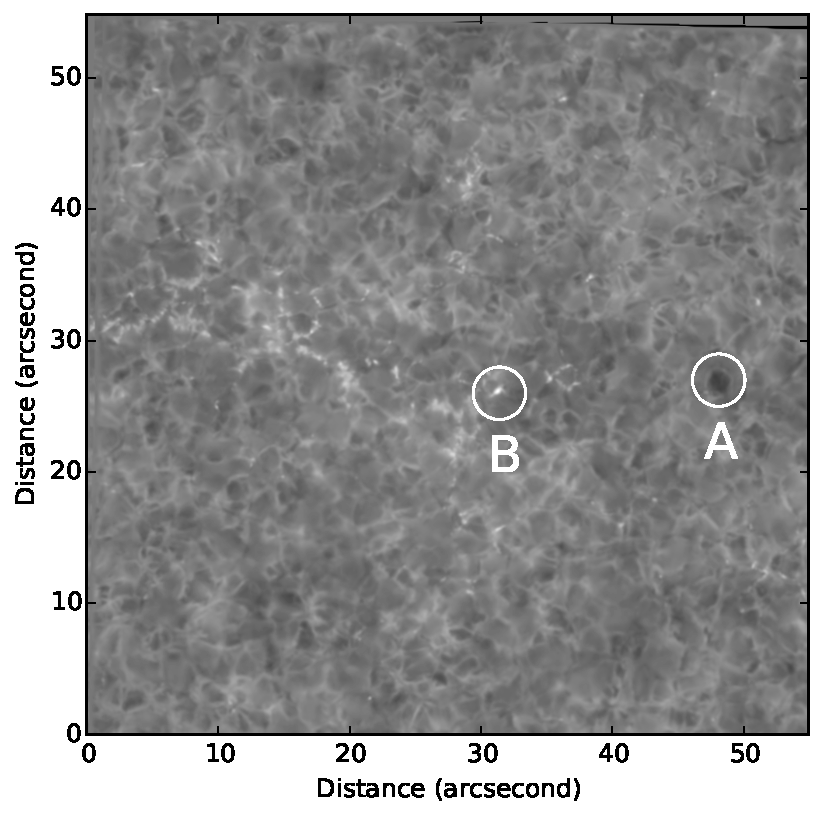
\includegraphics[width=\textwidth]{QS.pdf}
    	\caption{
    		Iron I ($630.2$ nm) image taken with the Swedish Solar Telescope on the $22^{\mathrm{nd}}$ of July 2012.
    		It shows some of the features that are present in the quiet Sun: a granule cell (A) and a magnetic bright point (B).
    	}
    	\label{fig:photosphere}        
    \end{figure}   
       
    The convective nature of the Sun has allowed us to infer the interior structure. 
    The reason for this is that turbulence within the convection zone creates an entire spectrum of acoustic waves, named \textit{p}-modes, where \textit{p} stands for pressure.
    \textit{p}-modes penetrate into the solar interior and at certain frequencies, the waves become standing.
    These can be measured on the photosphere, using line-of-sight Doppler images. 
    The mathematics used as a basis for this research is called spherical harmonics and allows \textit{p}-modes that are observed to be understood.
    The mode's overall properties are affected by the physical conditions where the maximum amplitude for that mode occurs. 
    This allows an image to be built up at every depth within the solar interior.
    For reviews on this topic, see \cite{annurev.aa.22.090184.003113} and \cite{RevModPhys.74.1073} for example.
    
    The dynamics of the photosphere is governed by two processes, convection as discussed above, and the solar magnetic field.
    Thus understanding how the magnetic field is structured within the photosphere is important. 
    The most common method employed in solar physics to measure the magnetic field, is to exploit the Zeeman effect.
    When atoms are subjected to a magnetic field, their spectral lines split as a function of field strength and polarization.
    Unfortunately, this effect can only really be used in the photosphere as the magnetic field present is strong enough to cause the Zeeman effect.
    However, many solar physicists have attempted measurements in various weak field areas \citep{1995ApJ...439..474M,1538-4357-613-2-L177,2008A&A...489L..57K}.
    These images are called solar magnetograms and they have revealed the basic magnetic field structure at the photosphere.
    The magnetic field is very weak ($\le 40$ Gauss) on average and is very sparse \citep{0004-637X-636-1-496,2011A&A...526A..60V}.
    This is referred to as the quiet Sun and is shown in Figure \ref{fig:photosphere}. 
    The dominating feature within this image is the granulation cells, which is the structures formed by convection can be seen clearly as well as several small features, which are discussed below. 
    Since granulation can be seen clearly, the magnetic field does not dominate within the quiet Sun, as it does in other regions.
    Figure \ref{fig:valc} demonstrates the semi-empirical mode of the quiet Sun atmosphere from \cite{1981ApJS...45..635V}, where the density and temperature of the atmosphere is blue and red respectively.
    This is typically termed the VALIIIc model and is used as the base atmosphere for many MHD simulations \citep{Mumford2015,GFME13a,fedun1,fedun2,2011AnGeo..29..883S,Wedemeyer2012,Vigeesh2012,0004-637X-743-1-14}.
    The important regions of the solar atmosphere can be seen clearly in this figure, such as the temperature minimum and transition region.
    
    \begin{figure}    
       	\centering
       	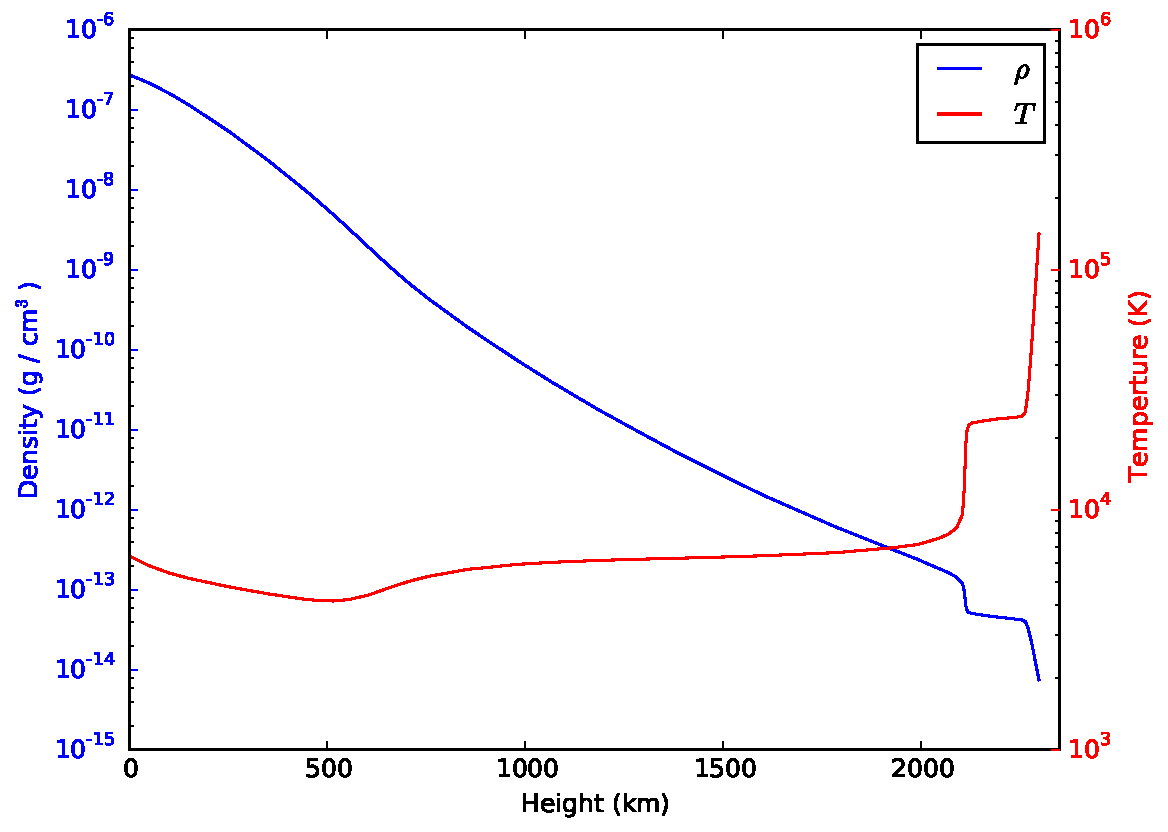
\includegraphics[width=\textwidth]{val3.pdf}
       	\caption{
       		     The VALIIIc \citep{1981ApJS...45..635V} model of the quiet Sun, density is blue and temperature is red.
       		     The temperature minimum region and the transition region can be seen clearly with these two parameters.
                 }
       	\label{fig:valc}        
    \end{figure} 
    
    Within the photosphere are small regions of concentrated magnetic field, named Magnetic Bright Points (MBPs).
    They are small-scale bright dots, as can be seen in Figure \ref{fig:photosphere}, in the circle labelled B.
    They are formed in the gaps between granule cells since the plasma flow drags the magnetic flux to high concentrations (>$1$ kG).
    The most likely reason for the increased brightness is that the flux tube has been evacuated of plasma.
    As such, observations of MBPs allow a glimpse into the top of the convection zone, which has a higher temperature than the photosphere and is brighter.
    One important factor about MBPs was the observation of Alfv\'en waves \citep{Jess2009,Taroyan2009}.
    This was able to supply enough energy to the corona to overcome the ``Coronal Heating problem'' (detailed in section \ref{corona}).
    
\subsubsection{Active regions}
    
    Active Regions (ARs) are areas of intense magnetic field concentrations on the Sun's surface.
    They are catalogued by the National Oceanic and Atmospheric Administration (NOAA) who  assign each AR a number.
    ARs vary in scale and in magnetic structure.
    Two of the most prevalent features within ARs are sunspots and magnetic pores.
    Furthermore, most ARs will contain magnetic features found in the quiet Sun and events that are believed to be a consequence of magnetic reconnection (spicules and Ellerman Bombs (EBs) for example). 
    Figure \ref{fig:AR} displays one such AR. 
    It consists of $3$ sunspots, taken as the AR is about to disappear off-limb.
    Circle A encloses one of the sunspots, but by use of a  different wavelength filter we can observe an EBs (B) and a jet event (C).
    The last two events are associated with magnetic reconnection \citep{2013SoPh..283..307N,2013A&A...560A..31N,2013ApJ...779..125N,2015ApJ...798...19N}.
     
    \begin{figure}
        \centering
        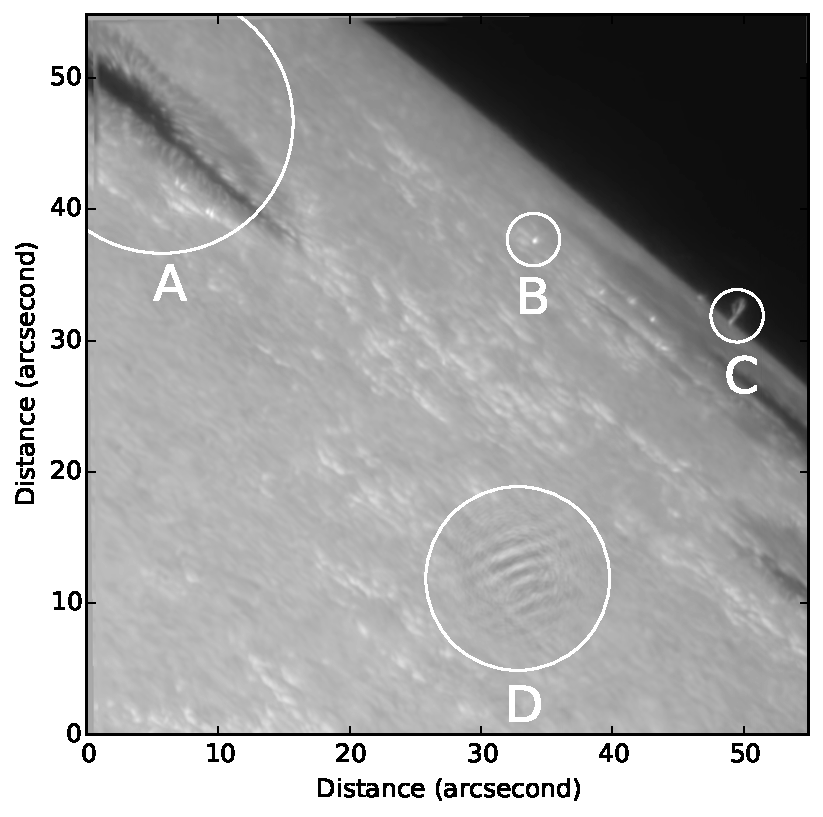
\includegraphics[width=\textwidth]{AR.pdf}
        \caption{
                 An image of an active region (NOAA 11504) sunspot taken with the Swedish Solar Telescope using the Crisp Imaging SpectroPolarimeter on the $21^{\mathrm{st}}$ June. 
                 The filter used is H$\alpha$ but into the far wings such that strong photospheric features can be observed.
                 It shows some of the features that are present in Active Regions; sunspot (A), Ellerman Bomb (B), a jet (C) and seeing effects (D).
              }
        \label{fig:AR}
     \end{figure}    

	ARs will form within a specific range of degree from the equator, typically $\pm$30$^\circ$.
	They most likely arise from a large coherent flux bundle that is formed depp in the convective zone.
	Magnetic buoyancy is the reason this bundle rises as a $\Omega$-shaped loop that breaks through the photosphere.
	Locally, the magnetic field is fragmented and convection is the mechanism that concentrates the emerging flux to form intense flux tubes, magnetic pores and sunspots.
	It can take up to 4 days for a well-developed AR to form and it is common that a sunspot group is surrounded by regions of enhanced brightness in the photosphere and in the corona, EUV and X-ray loops can be seen to be anchored in ARs.
	Many ARs will grow and reach a maximum size in about two weeks and sunspots will form during flux emergence but most disappear after a single rotation.
	The leader sunspot in an AR is called the p-spot (leader) and the last sunspot in the AR is called the f-spot (follower).
	The decay of an AR is takes longer than the growth stage and what is commonly seen is the slow cancellation and dispersal of magnetic flux as $\Omega$-loops submerge.
	Typically an AR are bipolar flux which are well-ordered into two islands of opposite polarity.
	
\subsubsection{Sunspots}

    Sunspots are the strongest magnetic field concentrations on the solar surface.
    A historical account of sunspots started from 1128 which is the oldest known chronicle by John of Worcester.
    With the invention of the telescope, as detailed at the start of this chapter, sunspots had been resolved into two parts by Galileo and Christoph Scheiner.
    They both showed that sunspots lie near the equator of the Sun.
    At the limb sunspot foreshortening was noted by Johnann Fabricius and he deduced that sunspots are on the surface of a moving sphere. 
    Alexander Wilson discovered that the side of a penumbra that is farthest from the limb is narrower.
    He deduced that a sunspot is a saucer-like depression (around 500-700 km) in the visible surface and this was named the Wilson effect.
    It was due to the colder, less-dense umbra being more transparent such that umbral light comes from a deeper level than the normal photosphere.

	With the naked eye, they appear as dark spots and are dark due to the partial inhibition by the magnetic field  of normal energy transport.
	However, with a good telescope, the sunspot structure is divided into two parts.
	The first is the dark central umbra with almost vertical magnetic field which is surrounded by a less-dark and highly filamentary penumbra with a characteristic pattern of bright and dark radial filaments and a weaker more horizontal inclined magnetic field.
	The umbral radius can make up to 50\% of the total sunspot radius.
	The brightness of the sunspot is dependant on wavelength but the total brightness (integrated over all wavelengths) is around 30\% of the quiet Sun.
	The temperature is 1000-2000 K less than the quiet Sun photosphere which implies that a substantial convective flux is required to maintain this brightness.
	The penumbra radiates 75-85\% of the quiet Sun photosphere and is only cooler by up to 400 K.
	Sunspots come in a range of shapes and sizes, with typical diamters that are 3.5 to 60 Mm and it was discovered that the lifetime of a sunspot is proportional to its area. 
	For example, a sunspot with diameter of 10 Mm will live for 2-3 days while a sunspot with a 60 Mm diameter will live up to 80-90 days.
	
	The magnetic field in the centre of the sunspot umbra is vertical and its strength increase while its brightness decreases with respect to size.
	The mean umbral magnetic field strength is 2.8 kG while it can be as weak er 1.5 kG and as strong as 6kG \citep{2006SoPh..239...41L}.
	The magnetic field strength decreases gradually with increasing radius from the centre and an average magnetic field over the entire sunspot is 1.2-1.7 kG.
	The penumbral inclination of the magnetic field increases with radius to a mean value of 70-80 degrees at the edge of the sunspot and the magnetic field weakens to 700-900 G.

	Sunspot groups are typically classified by the magnetic field polarity of the entire region.
	Typically the leader and follower sunspots have opposite polarity magnetic fields.
	For example, a uni-polar ($\alpha$-type) sunspot group makes up 46\% while bipolar ($\beta$-type) sunspots group make up 53\% and the remaining sunspot groups are very complex ($\gamma$-type).
	Figure \ref{fig:AR_Mag} show cases an example of a complicated sunspot group observed with National Aeronautics and Space Administration's (NASA) Solar Dynamics Observatory (SDO)'s Helioseismic and Magnetic Imager (HMI) instrument.
	The top image is a white light image while the bottom image is a magnetogram where blue is positive polarity and red is negative polarity magnetic field.
	These sunspot groups are the more likely ones to be the source of a large solar flare.
	Furthermore, $\delta$-type sunspots have an umbra that has an opposite polarity inside the same penumbra and large solar flares are common here as the magnetic gradients are high and the magnetic field is highly complex.
	
	Sunspots move faster than the surrounding plasma and this implies that they are most likely anchored below the surface where the rotation rate is faster.
	Sunspot groups tend to drift apart at a rate of 0.1$^\degree$ per day as the leader sunspot is at a lower latitude and will rotate faster since the Sun differential rotates.
	
	The umbra of a sunspot is far from uniform 
	It is known that dark nuclei that are around 15\% brightness of the queiet Sun photosphere
	
    Magnetic pores can be considered as smaller scale sunspots without a penumbra and thus are sometimes referred to, as ``naked umbra'' sunspots.
    They are intermediate flux concentrations between normal intenst flux tubes and sunspots.
	Magnetic pores have diameters that range from 0.7 to 7 Mm and the largest are bigger than the smallest sunspots.
	When compared to sunspots, they have a brightness that is 50\% of the quiet Sun photosphere and a central magnetic field strength of 1.8-2.3 kG and at the edge it has dropped to 1 kG.
    Due to their small size, magnetic pores have not been studied as much as sunspots since it took a new generation of solar telescopes in order to resolve them clearly.
    One example of a magnetic pore can be seen in Figure \ref{fig:chromosphere}, which is studied in Chapter \ref{chapter5}.
    This image is in the H$\alpha$ core which samples the chromosphere which is discussed in the next section.
		
	\begin{figure}
		\centering
		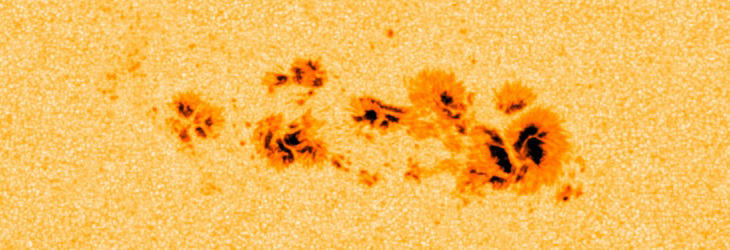
\includegraphics[width=\textwidth]{sunspot.jpg}\\
		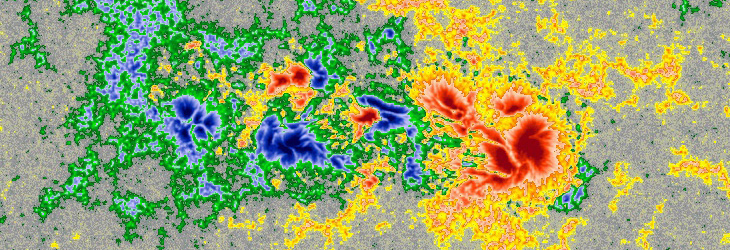
\includegraphics[width=\textwidth]{sunspot_magnetic.jpg}\\
		\caption{
				 An example of a very complex sunspot group with a $\gamma$ magnetic classification as seen by National Aeronautics and Space Administration's (NASA) Solar Dynamics Observatory (SDO)'s Helioseismic and Magnetic Imager (HMI) instrument.
				 This sunspot region was the source of a major X2.3 solar flare.
				 The top image shows us this sunspot region in visible light.
				 The bottom image is a so called ``magnetogram'' and shows the magnetic layout of a sunspot region.
				 The red colour indicates sunspots or areas with a negative polarity and the blue colour indicates areas with positive polarity sunspots.	
				}
		\label{fig:AR_Mag}
	\end{figure}

\cite{lrsp-2011-3}
\cite{2011IAUS..273....8R}

    Sunspot formation is a hotly debated topic (as many things are in solar physics).
    One current hypothesis about their formation is as follows.
    The magnetic field of the Sun is strongly polarised and with differential rotation, these magnetic fields lines become bunched together, increasing the local magnetic field strength.
    This effect creates a buoyancy force which slowly makes this newly created flux region rise towards the surface until it penetrates into the photosphere.
    It should be noted, however, that a complete understanding of how sunspots form has not yet been achieved and the mechanism is likely to be more complex than the one described above.
    In fairness of balance, other hypotheses are available.
    A more thorough review of the formation, evolution and unanswered questions relating to sunspots can be found in \cite{SAO}.

    While sunspots have been under near constant observation for several centuries.
    It was not until the mid 20$^{\mathrm{th}}$ century, that oscillations were observed within sunspots themselves \citep{OASO}.
    There are three main sunspot phenomena: 3-minute (5 mHz) and 5-minute (3 mHz) oscillations and running penumbral waves (RPWs).
    The first two are observed with a line-of-sight (LOS) analysis, i.e., frequency filtering using the Fast Fourier Transform (FFT) (which is covered in Chapter 2).
    However, there is some evidence to suggest the existence of longer period oscillations \citep{LPO,SOS,Chorley2011}.
    The source of the 5-minute oscillation is thought to be a result of forcing by the 5-minute \textit{p}-mode global solar oscillation \citep{OWS,WAUO}.
    The 5-minute oscillation are typically seen in lines which form low in the cool umbral photosphere and are moderately suppressed not only in the penumbra, but also in the chromospheric atmosphere above the umbra \citep{OASO}.
    The cause of the 3-minute oscillation is still unknown but there are two main theories: they are either standing acoustic waves which are linked to the resonant modes of the sunspot, or, they are low-$\beta$ slow magneto-acoustic waves guided along the ambient magnetic field \citep{UTMO,OWS,OASO,ORWS}.
    The 3-minute oscillation are seen in elements that form higher up, in the low chromosphere, and these are also moderately suppressed in the penumbra \citep{OASO}.
    However, it should not be assumed that the period of these waves form one finite peak in a power spectrum; generally, the immediate spectral area around these periods has several peaks clustered tightly together.
    A review of sunspot oscillations can be found in \cite{OASO} and a review of solar oscillations can be found in \cite{SO}.
    
    The solar cycle is on average a 11-year variation that the Sun undergoes.
    This cycle manifests itself as a variation in the number of sunspots, the amount of solar irradiance and the levels of other solar activity \citep{climate}.
    The polarity of the solar magnetic field inverts as well.
    So some suggest that the full solar cycle is 22 years, but the features that occur on the Sun seem to be independent of the current magnetic field polarity. 
    Each cycle has a solar maximum and a solar minimum.
    A solar maximum and a solar minimum refer to periods of maximum and minimum sunspot counts, respectively and cycles span from one minimum to the next.
    As the names suggest, there is a large amount of ARs and magnetic activity at a solar maximum, while this is reduced in a solar minimum.
    Each solar cycle can be seen in the amount of sunspots which are visible (i.e., the amount of ARs that form).
    This has been counted since the 17$^{\mathrm{th}}$ century and it is called the sunspot number catalogue \citep{Eddy18061976}.
    Figure \ref{fig:AR_Num} displays this catalogue with the raw count as the blue line and a running average in red.
    The main conclusion is that each cycle has a different duration and will produce a differing amount of sunspots.
    Since each solar cycle will differ in strength, the variation in the number of ``extreme'' events, such as flares and coronal mass ejections (CMEs) is observed.
    The reason is that these events require regions of strong magnetic field concentrations, i.e., ARs.
    So as the number of ARs decline, the possible regions that can cause flares or CMEs also decreases.
    Finally, the structure of the solar atmosphere will vary during each solar cycle as the magnetic field has an important effect on how the solar atmosphere is structured \citep{Sven}. 

    \begin{figure}
    	\centering
    	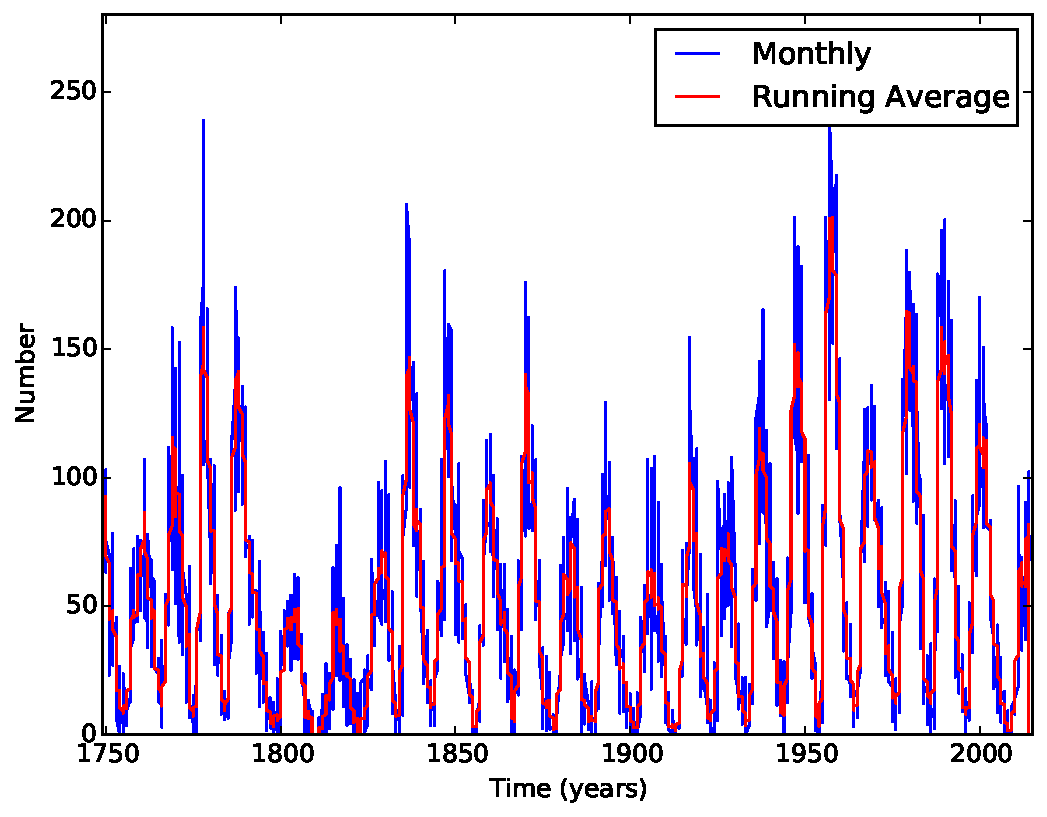
\includegraphics[width=\textwidth]{sunspot_number.pdf}
    	\caption{
	    		 The sunspot number record as it currently stands since continuous observations.  
    		     The eleven year solar cycle is clearly visible.
    	        }
    	\label{fig:AR_Num}
    \end{figure}   
            
    The solar cycle can directly impact the Earth's climate, as shown by the Maunder Minimum, which was an abnormally low amount of sunspots during the late seventeenth century and was the suspected cause of the Little Ice Age \citep{climate}.
    Earth, over the past five years was seeing another abnormal solar minimum, though it was not on the scale of the Maunder Minimum, it still had some effects on the climate.
    This was evidenced by the recent cold winters experienced by the northern hemisphere and it could influence the relationship between the atmospheric oscillations which affect the temperature of the northern hemisphere \citep{CWE,NAO,SCR}. 
   
\subsubsection{The chromosphere}
\label{chromo}

    \begin{figure}
        \centering
        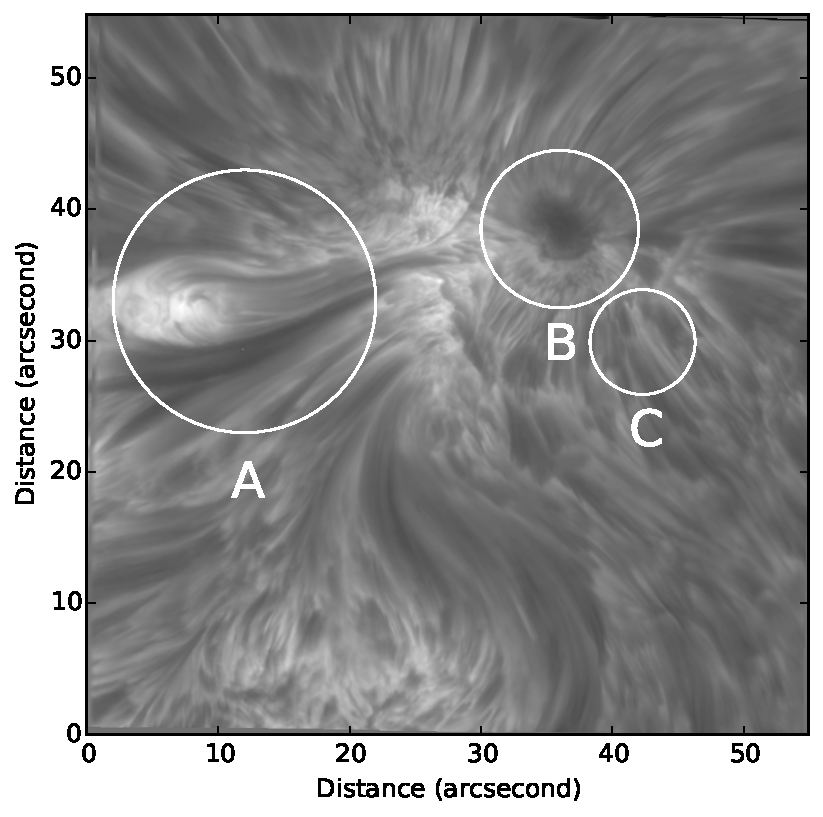
\includegraphics[width=\textwidth]{Chromo.pdf}
        \caption{
                 A H$\alpha$ line core image of Active Region NOAA 11510 observed on the 22$^{\mathrm{nd}}$ June 2012.
                 Here, this AR has a large pore that displays Running Penumbral waves (the focus of Chapter \ref{chapter5}).
                 Highlighted here are fibrils (A), the magnetic pore (B) and dynamic fibrils (C).
                 The complex nature of the chromosphere can be seen in detail and it still needs a full explanation.
                }
        \label{fig:chromosphere}
    \end{figure}   

    The next layer is visible from Earth when there is a total eclipse of the Sun, it is seen as an intense red region which got it the name, the chromosphere, from the Greek word ``chroma'', meaning colour.
    It is roughly $2$ Mm thick and is a highly complex layer.
    The temperature of the chromosphere increases with height and reaches around $20,000$ K at the boundary where it meets the next layer, the transition region.    
    The chromosphere is host to many small-scale structures that have been discovered due to the increasing optical resolution of solar telescopes over the past few decades.
    To observe the chromosphere from Earth, it is common to use either a H$\alpha$ filter, or a Ca II filter. 
    These are discussed in more detail later on in Chapter 2. 
        
    There are various names for these small-scale structures: spicules, fibrils, mottles and straws.
    The prevailing hypothesis is that there are two spicule types.
    Type I spicules are mainly seen in ARs but are scattered loosely elsewhere in the solar atmosphere.
    They can reach speeds up to $50$ km s$^{-1}$ and heights of $5$ Mm before falling back down, with typical lifetimes of $3$ to $10$ minutes, diameters of $120$ to $700$ km and temperatures of $10$ to $15$ kK.
    On disc, they are called dynamic fibrils and called mottles in the quiet Sun.
    Fibrils tend to be more elongated than mottles which are shorter.
    
    Type II spicules are located more often in the quiet Sun.
    They are faster (up to $150$ km s$^-1$), longer (up to $10$ Mm) and have a significantly reduced lifespan (up to $150$ s) when compared to Type I spicules.
    On disc, they are referred to as straws or more commonly Rapid Blue-shift Events (RBEs) \citep{Zaqarashvili2009}.
    Finally there is another fibril type that are long and mostly horizontal and longer-lived than dynamic fibrils.
    Some of these features are highlighted in Figure \ref{fig:chromosphere}.
    The circle A, has a good example of fibrils, long and fairly static, while circle C, shows dynamic fibrils which continually moved and swayed under our observation.
    
    These structures have been under investigation as a potential source of energy transport in the solar chromosphere.
    \cite{Morton2012} using ground-based observations discovered incompressible transversal motions for fibrils which match the ones observed for limb spicules which were interpreted as Alfv\'en waves \citep{DePontieu2007}.
    Further, fast compressive MHD waves were also observed.
    The estimation of the energy these waves carry is quite large but explaining how they dissipate this energy is unknown at this time.
    A review of oscillations in spicules can be found by \cite{Zaqarashvili2009}. 
      
    Running Penumbral Waves (RPWs), are a phenomenon discovered by \cite{Zirin1972} and \cite{Giovanelli1972}. 
    Observed in H$\alpha$ in sunspot penumbrae, they are seen as a wave train of enhanced darkness that moves from the umbra to the penumbra.
    They tend to be concentric and cover a large azimuthal angle.
    On average, they have a speed of $15$ to $20$ km s$^{-1}$ before slowing to $5$ to $7$ km s$^{-1}$ at the end of the penumbra.
    They have a typical period of $200$ to $300$ seconds. 
    Common interpretation is that much like the $3$-minute oscillations, they are slow magneto-acoustic wave propagating upwards along the inclined magnetic field and the radial outwards movement is actually a visual pattern \citep{UTMO,ORWS,OASO}.
    This is expanded on in Chapter \ref{chapter5}.
    
    Finally, we discuss the existence of a Moreton wave \citep{1960AJ.....65U.494M}.
    These are seen in H$\alpha$ wings as a dark and then a bright front.
    They travel away from flaring regions and are generally confined to a specific arc.
    They are more of a pulse than a wave and can travel at speeds up to $2000$ km s$^{-1}$.
            
\subsubsection{The transition region}

    Above the chromosphere, is a thin ($\approx100$ km) layer where the temperature rises rapidly from 20,000 K to 1,000,000 K.
    This is called the transition region.
    The rate of the increase is exponential and the density in this region decreases at a similar rate.
    In the bottom image of Figure \ref{fig:photosphere}, which displays the temperature and density of a semi-empirical model of the quiet Sun, this behaviour can be seen.
    This clearly means that the region is very non-uniform and \cite{tian2009solar} suggest that the height varies depending on what magnetic features are below the transition region.
    It cannot be observed from the surface of Earth, but can be from space-borne instruments sensitive to ultraviolet (UV) and extreme ultraviolet (EUV) light.
    
    Spicules, as discussed above, rise to large heights and it had been hypothesized that the TR would be a boundary.
    The spicule should hit the TR and create some form of a disturbance.
    These were discovered and called Transition Region Quakes (TRQs), found using the Extreme-Ultraviolet Imaging Spectrometer (EIS) instrument on-board the Japanese satellite Hinode.
    Coupled with MHD simulations, the disturbance was identified as a fast magneto-acoustic-gravity wave \citep{0004-637X-743-1-14}.
    These events further cement the link between the lower solar atmosphere and the higher regions.
    
\subsubsection{The corona}
\label{corona}

    The next layer is the outer atmosphere of the Sun is called the corona.
    It is most easily seen during a total solar eclipse, but also observable using a coronagraph \citep{markus2004physics}.
    The sheer scale of the corona is impressive.
    It extends many solar radii away from the solar surface and it is continuously expanding into the solar system which known as the solar wind.
    This entire region is called the heliosphere and this extends far past the orbit of Pluto.
    
    The average temperature of the corona is about 1-2 MK, however, it can reach temperatures as high as 8-10 MK \citep{markus2004physics}.
	The physical processes that account for the high temperature of the corona is still unknown, but two main hypotheses are in contention.
    The first one is called magnetic reconnection. 
    This process is where magnetic field changes its topology and the magnetic energy stored within the field is converted to kinetic and thermal energy and thus the plasma that is present in these reconnection regions will be heated. 
    The second one is MHD waves.
    The Sun creates a large amount of energy and the idea is that MHD waves can channel this energy from the convection zone through the various layers of the solar atmosphere and then into the solar corona.
	It requires that theses MHD waves are able to dissipate their energy into the plasma in order to heat this plasma.
    
    In all likelihood, a combination of these two main ideas will be the source behind coronal heating.
    This topic has been heavily researched for many decades and you can see reviews by \cite{erdelyi2004heating} and \cite{Parnell2012}.
    The most recent development has shifted the question, from ``how do you heat the corona?'' to ``how do you heat the chromosphere?'' \citep{Aschwanden2007}.
    
    The corona is host to many structures: X-ray bright points, plumes, prominences, streamers, coronal loops and coronal holes.
    When using a wavelength filter that samples higher temperature plasma ($\ge1$ MK), loop structures can be seen that rise several mega-meters in height.
    These are called coronal loops and they display a wide range of oscillations.
    See \cite{2010LRSP....7....5R} for a detailed review of coronal loops.
    Seismology of these loops has estimated the background quantities such as density and magnetic field strength of these loops (see \cite{2005RSPTA.363.2743D} or \cite{Banerjee2007} for a detailed review). 
    ARs  will also be the areas where flares or coronal mass ejections will originate from, since they contain large amounts of stored magnetic energy.
    
    These are the most spectacular events produced by the Sun.
    The amount of mass and energetic particles ejected can be considered scary, as these events have a direct impact on the Earth if the ejected material reaches Earth, from simply creating the aurora near the poles or in certain situations the disruption of radio transmissions, damage to satellites and electrical transmission lines.
    So it is important to understand the formation mechanism of these events so we can predict them and take measures to limit their damage.
    This is the realm of space weather research. 
    
    For a long time, it was hypothesised that MHD waves could not propagate into the corona due to the acoustic cut-off frequency.
    The launch of the Transition Region And Coronal Explorer (TRACE) space solar telescope changed this \citep{TRACE,TRACE1}.
    Numerous MHD oscillations where observed: damped transversal oscillations \citep{8007,2002A&A...394L..39G}, standing fast kink waves \citep{1999ApJ520880A,1999Sci...285..862N,1999SoPh..187..261S}, standing acoustic modes \citep{2003A&A...406.1105W}, fast sausage \citep{2001MNRAS.326..428W,2002MNRAS.336..747W,2003A&A...406..709K}, fast kink waves \citep{2005A&A...430L..65V}, propagating acoustic modes \citep{1997ApJ...491L.111O,2000A&A...355L..23D,2002A&A...393..649M} and torsional modes \citep{1998A&A...337..287E}. 
    This led to a large focus on coronal seismology which allows the estimation of the background properties of coronal loops using the observed properties of these waves.
    See a review on this topic by \cite{lrsp-2005-3}.
    Finally, EIT waves were discovered using the Extreme Ultraviolet Imaging Telescope (EIT) instrument onboard the Solar and Heliospheric Observatory (SOHO) space satellite \citep{1998GeoRL..25.2465T}.
    These are large single-pulsed propagating fronts which appear to move unhindered throughout the corona after a large-scale event (such as a flare).
    They are believed to be associated with Moreton waves.
        
    Overall, this has been a brief overview of the history of the Sun, its interior and atmosphere. 
    For a more detailed introduction to the Sun, see \cite{priest1984solar} or \cite{2014masu.book.....P} and see \cite{markus2004physics} for a detailed overview of the solar corona.
    
\section{MHD theory}

    The mathematical underpinning used in solar physics is called magnetohydrodynamics (MHD).
    It adds the effects of a magnetic field to the governing equations of fluid mechanics. 
    More accurately, it is the melding of Maxwell's equations to the Navier-Stokes equations.
    This is credited to Hannes Alfv\'en, who won a Nobel Prize in Physics for this major contribution to science \citep{1942Natur.150..405A,erdelyi2007}.

\subsection{MHD equations}

    There are several equations that form the core of MHD and are solved in many different magnetic configurations. 
    The ultimate aim is to understand how these configurations will evolve in time or how they react to external factors.
    Further, they are solved to find out what kind of waves these configurations can support and how these waves perturb the system. 
    The MHD equations include many physical effects, however, we have taken the ideal assumption; adiabatic, inviscid, non-radiative, no thermal conduction and no resistivity.
    This is ideal MHD and the resulting equations are,
    \begin{align}                                                         
        \dfrac{\partial \rho }{\partial t} + \nabla \cdot (\rho \boldsymbol{\mathrm{v}}) =       
        0,\tag{Mass Conservation}\\                                  
        \rho \dfrac{\mathrm{D}\boldsymbol{\mathrm{v}}}{\mathrm{D}t} =
        -\nabla p + \dfrac{1}{\mu}(\nabla \times \boldsymbol{\mathrm{B}}) \times \boldsymbol{\mathrm{B}} + \rho \boldsymbol{\mathrm{g}},\tag{Equation of Motion}\\
        \dfrac{\mathrm{D}}{\mathrm{D}t} \left(\dfrac{p}{\rho^\gamma} \right)  = 0,\tag{Energy Equation}\\       
        \dfrac{\partial \boldsymbol{\mathrm{B}}}{\partial t} = \nabla \times (\boldsymbol{\mathrm{v}} \times \boldsymbol{\mathrm{B}}),\tag{Induction Equation}               
    \end{align}
    subject to
    \begin{align}
        \nabla \cdot \boldsymbol{\mathrm{B}} = 0,\tag{Solenoid Equation}\\
        p = \mathrm{k_B} \dfrac{\rho}{\mathrm{m}} \mathrm{T},\tag{Ideal Gas Law}\\  
        \boldsymbol{\mathrm{E}} = - \boldsymbol{\mathrm{v}} \times \boldsymbol{\mathrm{B}},\tag{Ohm's Law}\\
        \boldsymbol{\mathrm{j}} = \nabla \times \boldsymbol{\mathrm{B}}/ \mu.\tag{Electric Current}                          
    \end{align}
    Here $\rho$ is the density, $\boldsymbol{\mathrm{v}}$ is the velocity, $\frac{\mathrm{D}}{\mathrm{D}t}$ is the convective derivative $\left(\frac{\partial}{\partial t} + (\boldsymbol{\mathrm{v}}\cdot\nabla)\right)$, $p$ is the pressure, $\gamma$ is the ratio of specific heats ($5/3$ for an ideal mono-atomic gas), $\boldsymbol{\mathrm{B}}$ is the magnetic field, $\mathrm{k_B}$ is Boltzmann's constant, $\mathrm{m}$ is the mass, $\mathrm{T}$ is the temperature, $\boldsymbol{\mathrm{E}}$ is the electric field, $\boldsymbol{\mathrm{j}}$ is the current density and $\mu$ is the vacuum permeability. 

    There are actually eight partial differential equations for eight variables.
    Both $\boldsymbol{\mathrm{v}}$ and $\boldsymbol{\mathrm{B}}$ have three components each and we have the density and temperature.
    From this, the typical recourse is to examine the case of small perturbations for the MHD quantities, i.e.,
    \begin{align*}                                                         
        \boldsymbol{\mathrm{B}} &= \boldsymbol{\mathrm{B}}_0 + \boldsymbol{\mathrm{B}}_1(\boldsymbol{r},t)\\               
        \boldsymbol{\mathrm{v}} &= \boldsymbol{0} + \boldsymbol{\mathrm{v}}_1(\boldsymbol{r},t)\\               
        p &= p_0 + {p_1}(\boldsymbol{r},t)\\               
        \rho &= \rho_0 + {\rho_1}(\boldsymbol{r},t).\\              
    \end{align*}
    Here, subscripts are used to separate out the background ($\mathrm{B}_0$) and perturbation ($\mathrm{B}_1$) quantities.
    There is assumed to be no background flow and that all perturbations are much smaller than the background value (e.g., $\mathrm{B}_0 \gg \mathrm{B}_1$).      
    This leads to the linearised ideal MHD equations,
    \begin{align}                                                         
    \dfrac{\partial \rho_1 }{\partial t} + (\boldsymbol{\mathrm{v}}_1 \cdot \nabla)\rho_0 + \rho_0 (\nabla \cdot \boldsymbol{\mathrm{v}}_1) =       
    0,\tag{Mass Conservation}\\                                  
    \rho_0 \dfrac{\partial \boldsymbol{\mathrm{v}}_1}{\partial t} =
    -\nabla p_1 + \dfrac{1}{\mu}(\nabla \times \boldsymbol{\mathrm{B}}_1) \times \boldsymbol{\mathrm{B}}_0 + \rho_1 \boldsymbol{\mathrm{g}},\tag{Equation of Motion}\\
    \dfrac{\partial p_1}{\partial t} + (\boldsymbol{\mathrm{v}}_1 \cdot \nabla)p_0 - c_s^2 \left( \dfrac{\partial \rho_1}{\partial t} + (\boldsymbol{\mathrm{v}}_1 \cdot \nabla)\rho_0 \right) = 0,\tag{Energy Equation}\\       
    \dfrac{\partial \boldsymbol{\mathrm{B}}_1}{\partial t} = \nabla \times (\boldsymbol{\mathrm{v}}_1 \times \boldsymbol{\mathrm{B}}_0),\tag{Induction Equation}\\
    \nabla \cdot \boldsymbol{\mathrm{B}}_1 = 0, \tag{Solenoid Equation}               
    \end{align}
    where we can define the first characteristic speed in MHD, the sound speed, $c_s^2 = {\gamma p_0}/{\rho_0}$.
    There is another important characteristic speed and that is the Alfv\'{e}n speed, $c_A^2 = {\mathrm{B}_0^2}/{\sqrt{\rho_0}}$.
    These equations need to then be applied to an equilibrium and, since the focus is sunspots and magnetic pores, a cylindrical flux tube is the ideal choice.
    
\subsection{MHD waves in cylindrical flux tubes}

    To understand the observed oscillations in sunspots and pores, it is important to investigate the nature of oscillations within an idealised model of these structures.
    However, before this occurs, a quick comment on MHD waves in a uniform infinite plasma atmosphere.
    Table \ref{tab:uniform_medium} summarises how MHD wave mode behaves within the traditional model used to explain MHD to undergraduates.
    This model is a uniform unbounded (i.e., infinite) atmosphere with a background magnetic field that is purely vertical.
    Three wave modes are present in this model, the Alfv\'{e}n mode, the fast mode and the slow mode.
    To summarise, the Alfv\'{e}n perturbs the velocity in a perpendicular direction to its propagation direction. 
    It also only propagates along the magnetic field lines and not perpendicular.
    For the fast and slow wave mode, the velocity perturbation is not perpendicular to the angle of propagation.
    The important distinction between the fast and slow mode in this model is that the slow mode does not propagate perpendicular to the background magnetic field, while the fast mode is isotropic.
    The effect of plasma-$\beta$ in this regime is to simply change the speed at which the slow and fast mode will propagate at.  
    This results tend to be summarised in Friedrich diagrams. 
    In the context of a cylindrical tube, only the fast and slow modes are discussed.
             
    \begin{sidewaystable}
	    \centering
		\begin{tabular}{lccc}
   			&			& $\beta \gg 1$, $\va \ll \vs$	&   $\beta \ll 1$, $\va \gg \vs$ 	 	\\
   			\vspace{-3mm} \\
   			\hline
   			\hline
   			\vspace{-2mm} \\
   			& $\bm{\mathrm{k}} || \Beq$		& Alfv\'{e}n wave, $\vph^2 \sim \va^2$		& Alfv\'{e}n wave, $\vph^2 \sim \va^2$	\\
   			$\bm{\mathrm{k}} \cdot \boldsymbol{\mathrm{v}}_1 = 0$	&					&									&								\\
   			& $\bm{\mathrm{k}} \perp \Beq$	& Alfv\'{e}n wave -- does not propagate 		& Alfv\'{e}n wave -- does not propagate	\\
   			\vspace{2mm} \\
   			& 					& Fast wave, $\vph^2 \sim \vs^2$	 		& Fast wave, $\vph^2 \sim \va^2$		\\
   			& 					& approximately isotropic	 			& approximately isotropic		\\
   			& $\bm{\mathrm{k}} || \Beq$		& magnetic and kinetic pressure in phase	& magnetic and kinetic pressure in phase	\\
   			& 					& Slow wave, $\vph^2 \sim \va^2$	 		& Slow wave, $\vph^2 \sim \vs^2$		\\
   			& 					& magnetic and kinetic pressure out of phase	& magnetic and kinetic pressure out of phase	\\
   			$\bm{\mathrm{k}} \cdot \boldsymbol{\mathrm{v}}_1 \neq 0$&					&									&							\\
   			& 					& Fast wave, $\vph^2 \sim \vs^2$	 		& Fast wave, $\vph^2 \sim \va^2$		\\
   			& $\bm{\mathrm{k}} \perp \Beq$	& approximately isotropic	 			& approximately isotropic		\\
   			& 					& magnetic and kinetic pressure in phase	& magnetic and kinetic pressure in phase	\\
   			& 					& Slow wave -- does not propagate	 		& Slow wave -- does not propagate		\\
   			\hline
   			~&~&~ \\
   		\end{tabular}
		\caption{
				 Phase speeds of the slow, fast and Alfv\'{e}n waves for a uniform unbounded magnetised plasma.
			     Adapted from \cite{jess2015multiwavelength}.
			    }
		\label{tab:uniform_medium}
     \end{sidewaystable}
     
    The most iconic investigation into this was undertaken by Edwin and Roberts in 1983 \citep{WPMC}.
    Their analysis is based on the non-slender flux tube, where the tube radius is greater or equal to the wavelength of the oscillations.
    Further it ignores the effects of gravity (i.e., the stratification of the atmosphere), which is important when the wavelength is comparable to the atmospheric scale height and in the photosphere this is the case \citep{LNLMHD}. 
    It is important to note that in thin flux tubes, there are two other characteristic wave speeds.
    One is a subsonic, sub-Alfv\'{e}nic speed, $c_T$ (defined later on), and the other is the ``mean'' Alfv\'{e}n speed, $c_k$.

    The model is as follows, a cylindrical magnetic flux tube of radius $a$ with its own density ($\rho_0$), pressure ($p_0$) and magnetic field ($\mathrm{B}_0\textbf{\^{z}}$) is embedded in a magnetic environment with a similar profile ($\mathrm{B}_e \textbf{\^{z}}$, $\rho_e$ and $p_e$).   
    The density and pressure are uniform throughout the medium.
    The top image of Figure \ref{fig:fluxtube} is a schematic drawing of this model. 
        
    \begin{figure}
        \centering
        \begin{subfigure}[b]{0.75\textwidth}
            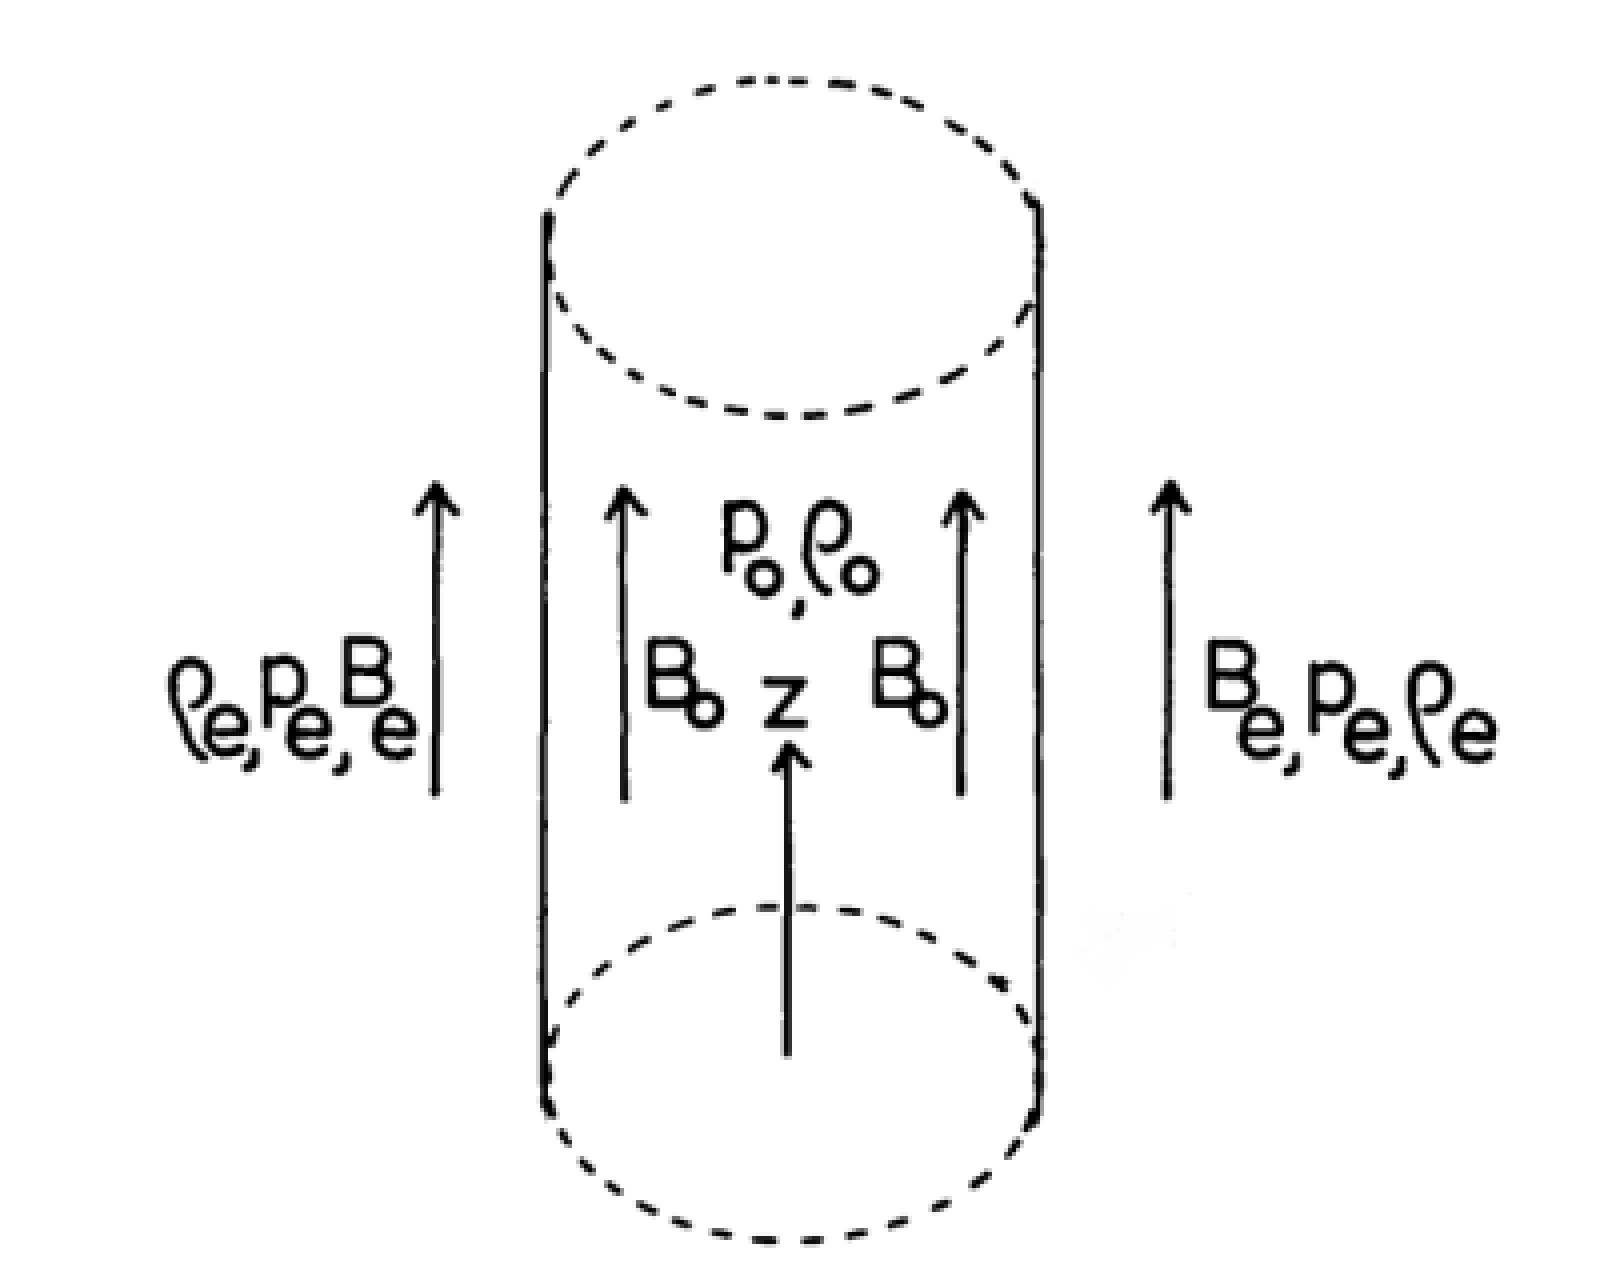
\includegraphics[width=\textwidth]{Fluxtube}
        \end{subfigure}\\~\\
        \begin{subfigure}[b]{0.65\textwidth}
            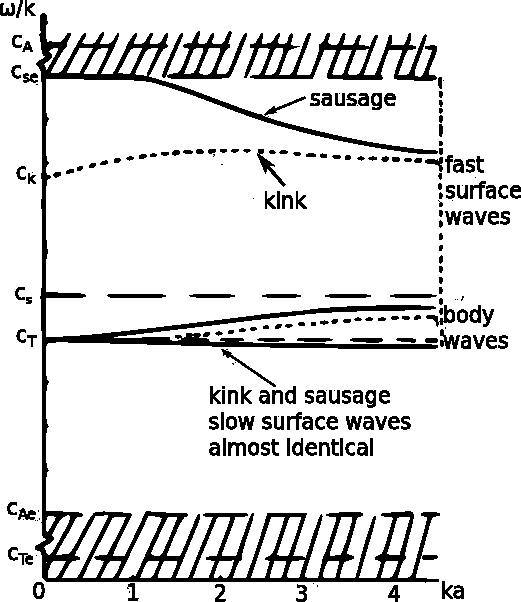
\includegraphics[width=\textwidth]{dispersion}
        \end{subfigure}
        \caption{
                \textit{(top)} The equilibrium conditions used to model wave behaviour in a magnetic flux tube.
                Image is a modified version of Figure 1 from \cite{WPMC}.
                \textit{(bottom)} The dispersion relationship derived from the MHD equations under photospheric conditions ($c_A > c_{se} > c_k > c_{Ae} $).
                The hatched areas are the excluded  values of $\omega$ and $ka$.
                Image is a modified version of Figure 2 from \cite{WPMC}.
                }
        \label{fig:fluxtube}
    \end{figure}
    
    This is the starting point for deriving the dispersion relation for MHD waves in a magnetic flux tube.
    It is assumed that this system is in equilibrium.
    Perturbations to the equilibrium conditions then add extra terms to the ideal MHD equations (the equations above).
    By introducing the Fourier decomposition of the perturbations, they show that the amplitude term is the Bessel equation.
    When bound on the axis of the cylinder ($r=0$), two solutions exist for either the body or surface wave.
    In the external atmosphere, the assumption of no propagation of energy away from or towards the cylinder allows the solution for the amplitude to be found for the external atmosphere.
    Further, the kinetic and magnetic energy density tend to zero as $r\rightarrow\infty$.
    Continuity at the boundary ($r=a$) has to be kept (radial velocity component $v_r$, and the total pressure) which yields the dispersion relations for surface waves and body waves \citep{WPMC}.
    These are,
    \begin{align}
        \rho_0 (k^2 c_A^2 - \omega)m_e \dfrac{K_n^\prime(m_e a)}{K_n(m_e a)} &= \rho_e (k^2 c_{Ae}^2 - \omega)m_0 \dfrac{I_n^\prime(m_0 a)}{I_n(m_0 a)} \tag{Surface, m$_0^2 > 0$} \\
        \rho_0 (k^2 c_A^2 - \omega)m_e \dfrac{K_n^\prime(m_e a)}{K_n(m_e a)} &= \rho_e (k^2 c_{Ae}^2 - \omega)n_0 \dfrac{I_n^\prime(n_0 a)}{I_n(n_0 a)} \tag{Body, m$_0^2 = -n_0 < 0$} 
    \end{align}
    where, $K_n$ and $I_n$ are Bessel functions of order n, $K_n^\prime$ and $I_n^\prime$ are the derivatives of the Bessel functions, $m_0$ and $m_e$ are the internal and external wavenumber, defined as, $$\dfrac{(k^2 c_{s}^2 - \omega^2)(k^2 c_{A}^2 - \omega^2)}{(c_{s}^2 + c_{A}^2)(k^2 c_{T}^2 - \omega^2)},$$ and $c_{T}$ is the tube speed, $$c_{T} = \dfrac{c_s^2 c_A^2}{c_s^2 + c_A^2}.$$
    Finally, these dispersion relations are solved under photospheric conditions (plasma-$\beta << 1$, such that, $c_A > c_{se} > c_k > c_{Ae} $) and the solutions are plotted at the bottom of Figure \ref{fig:fluxtube}.
        
    These dispersion relations are important as they detail the way in which waves propagate through numerous flux tube sizes.
    It shows the limits of the wave solutions indicating in what regimes they cannot exist.
    Surface waves are dispersive as their phase speed depends on the wavenumber.
    There are slow body waves which are both sausage, kink and fluting modes and these modes have a phase speed between the tube and sound speeds.
    Slow surface waves have phase speeds close to the tube speed. 
    There is also a surface wave with a phase speed close to the kink speed and another surface wave near the sound speed.
    If one can measure the phase speed of an observed wave and the $ka$ of the flux tube, one can also likely identify the observed waves.
    This has been attempted by \cite{2015A&A...579A..73M}.
    
    One factor that has been neglected is the mode number ($n$), its value governs the way in which the wave perturbs the flux tube.
    This gives us the name: sausage ($n=0$), kink ($n=1$) and fluting ($n>1$).
    These different wave modes cause characteristic physical effects which can be used to identify each different wave mode.
    
    Figure \ref{fig:tube} shows the physical changes to the flux tube, caused by each different wave mode.
    Below, when a quantity is talked about, the focus is on the perturbation of that quantity.
    The first diagram (labelled a), shows how the slow wave affects the flux tube. 
    The velocity is primarily longitudinal.
    Further, when the flux tube contracts the density decreases in that region indicating a phase difference of $\pi$, but this is also the same phase difference for the cross-sectional area and total intensity.
    The second diagram (labelled b), shows the fast sausage mode.
    The velocity is primarily radial and when the flux tube contracts the density in that region increases unlike the slow sausage mode.
    This means that the cross-sectional area and total intensity are in phase, as well as the magnetic field.
    These diagrams have been improved over time and movies have been created which can be found within several papers \citep{Morton2012,jess2015multiwavelength} and online sources (\url{http://www2.warwick.ac.uk/fac/sci/physics/research/cfsa/research/wpc/vis/} or \url{http://swat.group.shef.ac.uk/fluxtube.html}).
    Finally, the last diagram (labelled c) shows the kink wave mode.
    It is non-compressible (to the first order linear limit, long wavelength approximation) and perturbs the flux tube axis.
    This makes it very difficult to identify unless it is possible to isolate the central axis of the flux tube.
    This is quite difficult for a sunspot or magnetic pore, but it has been done for spicules and fibrils and  kink and Alfv\'en waves have been observed (see section \ref{chromo} for more details).
    
    \begin{figure}
    	\centering
    	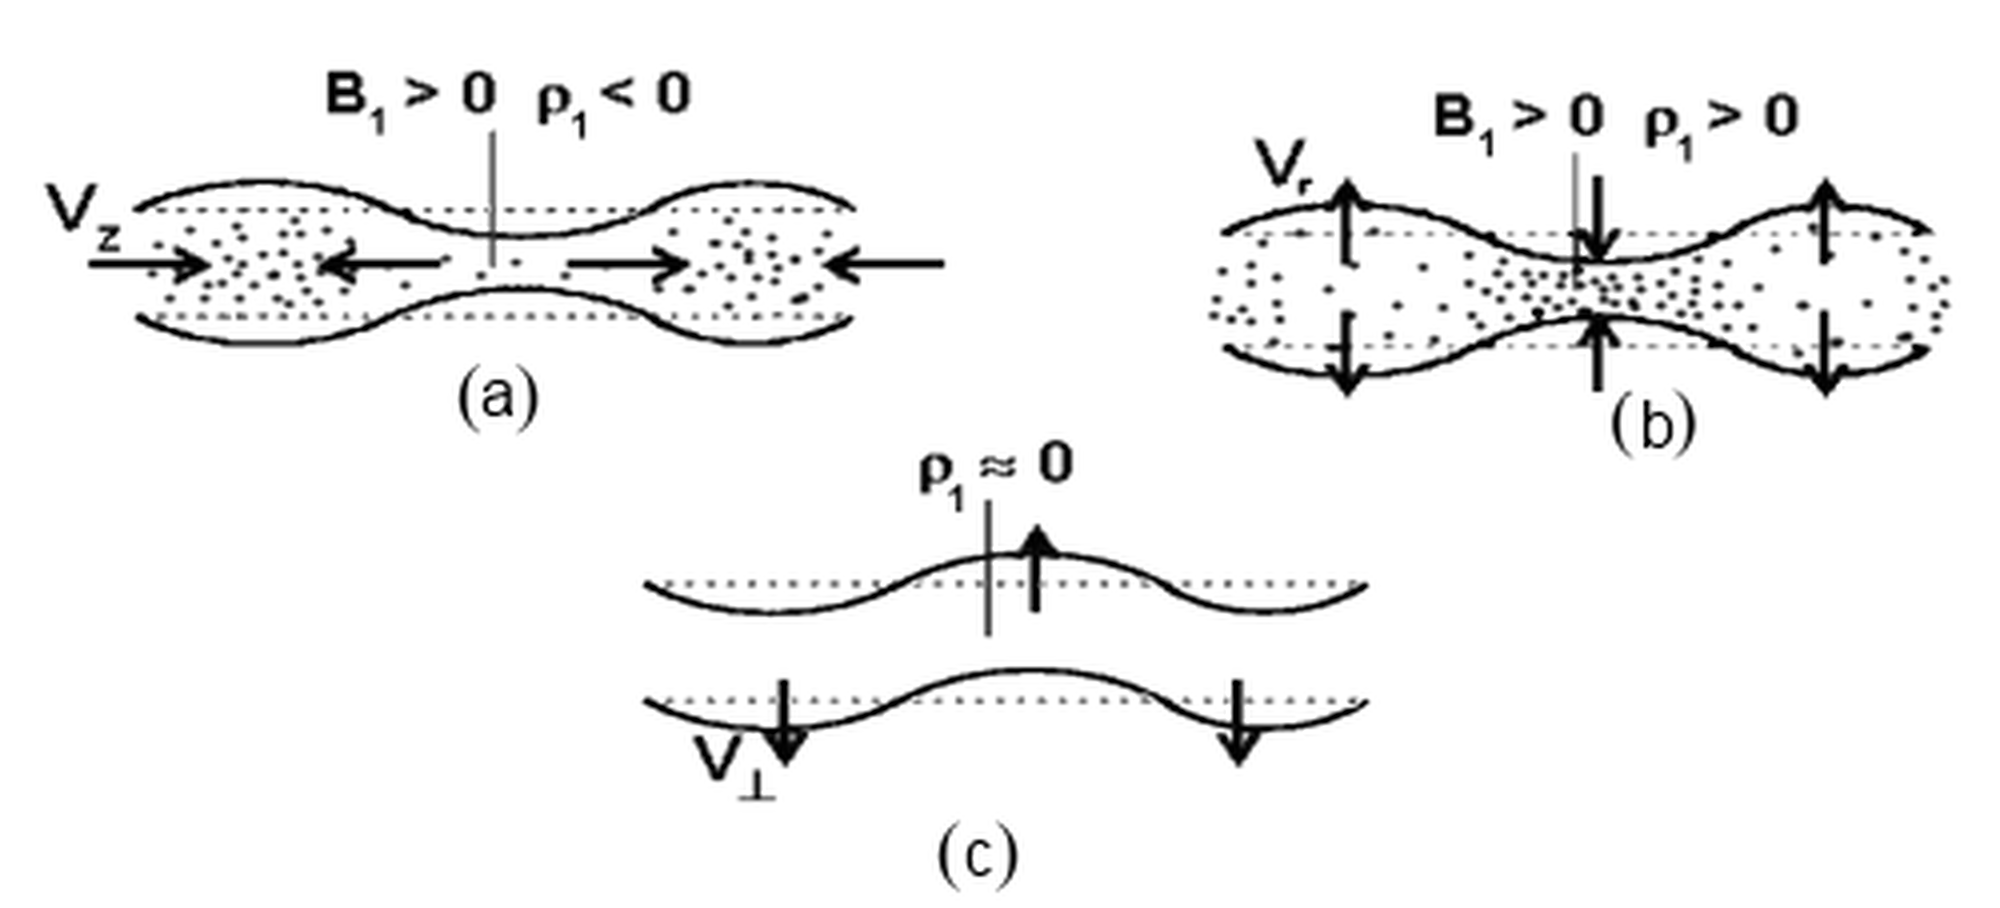
\includegraphics[width=\textwidth]{tube}
    	\caption{
    		The physical effects that each type of wave has on the flux tube.
    		(a) The slow magneto-acoustic waves (slow sausage mode) which cause anti-phase behaviour between the intensity and the magnetic field.
    		(b) The fast magneto-acoustic waves (fast sausage mode) which cause in phase behaviour between the intensity and the magnetic field.
    		(c) The fast magneto-acoustic waves (fast kink mode) which cause no magnetic field perturbations but cause $\pi/2$ phase behaviour between the intensity and velocity perturbation.
    		Image is a modified version of Figure 1 from \cite{CLOO}.
    	}
    	\label{fig:tube}
    \end{figure}
   
	While these are toy arguments and descriptions, these phase relations have been derived by several authors \citep{PMHDW,Moreels2013,Moreels2013b,2015A&A...579A..73M}.
    They have taken complex models of embedded flux tubes to derive an almost full set of phase relations for many of the MHD wave modes and whether they are standing or propagating.
	The main conclusions from \cite{Moreels2013} and \cite{Moreels2013b} is that fast and slow sausage modes have a different phase behaviour; namely that slow modes have an in phase behaviour (i.e., $0$ degrees phase difference between the cross-sectional area and the Lagrangian intensity oscillations), while fast modes have an anti-phase behaviour (i.e., $180$ degrees phase difference between the cross-sectional area and the Lagrangian intensity oscillations).
    Throughout all of this thesis we use the Lagrangian intensity variations, i.e., the intensity variations when following the motion of the plasma, when discussing the intensity. 
     
    Table \ref{tab:phase} summarises the phase relations between the intensity, Doppler velocity, magnetic field and for the cross-sectional area and intensity for each wave type and whether it is a standing or propagating wave.
    This table contains the information that will be used later on in this thesis, in order to identify the observed oscillations which occur within the numerous magnetic structures analysed. 
    Since the focus has been on compressive perturbations, kink waves are neglected from this point onwards, as are Alfv\'en waves.
    However, see these recent review of both of these waves with regards to theory and observations \citep{Mathioudakis2013,jess2015multiwavelength}.
    It is important to note that the focus has been exclusively on MHD sausage waves within this thesis.
  
    \begin{table}
        \centering
        \begin{tabular}{l|c|c|c|c}
            &$\phi_{\mathrm{B}}-\phi_{\mathrm{v}}$&$\phi_{\mathrm{v}}-\phi_{\mathrm{I}}$&$\phi_{\mathrm{I}}-\phi_{\mathrm{B}}$&$\phi_{\mathrm{S}}-\phi_{\mathrm{I}}$ \\ \hline\hline
        Slow sausage propagating        & $\pi$ & 0 & $\pi$ & 0 \\
        Slow sausage standing           & $\pm\pi/2$ & $\pm\pi/2$ & $\pi$ & 0 \\
        Fast sausage propagating$^6$    & [0,$\pi$] & [$-\pi/2$,0] & [$-\pi/2$,0] & $\pi$ \\
        Fast sausage standing$^6$       & $\pm\pi/2$ & $\pm\pi/2$ & [0,$\pi$] & $\pi$  \\
        Fast kink propagating       	& $\pm\pi/2^3$ & $N/A^4$ & $N/A^4$ & $N/A^4$ \\
        Fast kink standing          	& [$\pi/2^1,\pi^2$] & $N/A^4$ & $N/A^4$ & $N/A^4$ \\ \hline
        \end{tabular}
        \caption{
            Shows the phase differences between three observables: the intensity, Doppler velocity and the magnetic field for each type of MHD wave and whether the wave is standing (S) or propagating (P).
            1 - Wave propagating anti-parallel to the magnetic field.
            2 - Wave propagating parallel to the magnetic field. 
            3 - Depending on the distance to the reflection boundary.
            4 - Kink modes are incompressible and thus have zero intensity fluctuations.
            5 - Fast sausage mode has zero LOS velocity fluctuations.
            6 - Surface mode only.
            Collated from these authors, \cite{CLOO,PMHDW,Moreels2013,Moreels2013b,2015A&A...579A..73M}}
        \label{tab:phase}
    \end{table}
    
	The previously derived theory \citep{Moreels2013,Moreels2013b,2015A&A...579A..73M,jess2015multiwavelength} gives an insight into the observational signatures that MHD sausage waves will exhibit within a magnetic waveguide.
	While the base signature will be the change of the cross-sectional area with respect to time and that this signal should be either in phase or out of phase with the total intensity signal. 
	What is missing from this, is whether the two MHD sausage modes (slow and fast) have characteristics that will either it easy or difficult to observe.
    \cite{Moreels2013} suggest that the fast MHD sausage mode, in photospheric conditions, should be able to perturb the radius up to 20\%.
    For the slow MHD sausage mode, the type of wave becomes important.
    For waves within flux tubes, there are two wave types: body and surface.
	For the slow MHD sausage surface mode, the perturbation amplitude is very small, below the resolution of current telescopes.
	However, the slow MHD sausage body mode, should be able to perturb the radius up to 10\%.
	The reason for this difference between the slow and fast mode is that the dominant velocity perturbation is longitudinal for the slow mode while it is radial for the fast mode.
    \cite{jess2015multiwavelength} suggest that the fast MHD sausage mode has a larger cross-sectional area perturbation as well as stronger density perturbations compared to the MHD slow sausage mode.
    Overall, the current research suggests that the effect of MHD sausage modes is observable with the current generation of ground-based telescopes.